\documentclass[border=3pt]{standalone}
\usepackage{tikz}
\usetikzlibrary{braids,calc}

\begin{document}

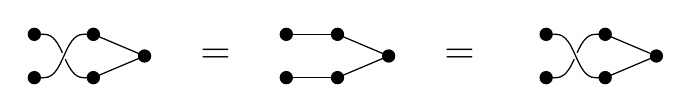
\begin{tikzpicture}[
  baseline=(current bounding box.center),
  dot/.style={circle, fill, inner sep=1.7pt},
  line/.style={line width=0.45pt}
]

%================================================
% LEFT SIDE:  \mu \circ \beta
%================================================
\pic[
  rotate=90,
  name=brL,
  braid/.cd,
  number of strands=2,
  width=5.5mm,
  crossing height=5.5mm,
  border height=1mm,
  every strand/.style={line width=0.45pt}
] at (0,0) {braid={s_1}};

\coordinate (mL) at ($(brL-1-e)!0.5!(brL-2-e)+(0.65cm,0)$);

\draw[line] (brL-1-e) -- (mL);
\draw[line] (brL-2-e) -- (mL);

\foreach \i in {1,2}{
  \node[dot] at (brL-\i-s) {};
  \node[dot] at (brL-\i-e) {};
}
\node[dot] at (mL) {};

% first equals sign
\node at ($(mL)+(0.9cm,0)$) {\Large $=$};

%================================================
% MIDDLE:  \mu
%================================================
\coordinate (a1) at ($(mL)+(1.8cm,0.275cm)$);
\coordinate (a2) at ($(mL)+(1.8cm,-0.275cm)$);
\coordinate (b1) at ($(a1)+(0.65cm,0)$);
\coordinate (b2) at ($(a2)+(0.65cm,0)$);
\coordinate (mM) at ($(b1)!0.5!(b2)+(0.65cm,0)$);

\draw[line] (a1) -- (b1);
\draw[line] (a2) -- (b2);
\draw[line] (b1) -- (mM);
\draw[line] (b2) -- (mM);

\foreach \p in {a1,a2,b1,b2,mM}
  \node[dot] at (\p) {};

% second equals sign
\node at ($(mM)+(0.9cm,0)$) {\Large $=$};

%================================================
% RIGHT SIDE:  \mu \circ \beta^{-1}
%================================================
\pic[
  rotate=90,
  name=brR,
  braid/.cd,
  number of strands=2,
  width=5.5mm,
  crossing height=5.5mm,
  border height=1mm,
  every strand/.style={line width=0.45pt}
] at ($(b2)+(0.65cm,0)+(2.0cm,0)$) {braid={s_1^{-1}}};

\coordinate (mR) at ($(brR-1-e)!0.5!(brR-2-e)+(0.65cm,0)$);

\draw[line] (brR-1-e) -- (mR);
\draw[line] (brR-2-e) -- (mR);

\foreach \i in {1,2}{
  \node[dot] at (brR-\i-s) {};
  \node[dot] at (brR-\i-e) {};
}
\node[dot] at (mR) {};

\end{tikzpicture}

\end{document}